%% LyX 2.3.0 created this file.  For more info, see http://www.lyx.org/.
%% Do not edit unless you really know what you are doing.
\documentclass[english]{paper}
\usepackage[T1]{fontenc}
\usepackage[latin9]{inputenc}
\usepackage{geometry}
\geometry{verbose,tmargin=0.7in,bmargin=0.5in,lmargin=0.75in,rmargin=0.75in}
\usepackage{babel}
\usepackage{amsmath}
\usepackage{amssymb}
\usepackage{graphicx}
\usepackage[unicode=true,
 bookmarks=true,bookmarksnumbered=false,bookmarksopen=false,
 breaklinks=false,pdfborder={0 0 1},backref=false,colorlinks=false]
 {hyperref}
\hypersetup{pdftitle={EE5600 Assignment 3},
 pdfauthor={Joshua Saunders},
 pdfsubject={Linear Systems Analysis}}

\makeatletter
%%%%%%%%%%%%%%%%%%%%%%%%%%%%%% User specified LaTeX commands.
\renewcommand{\labelenumi}{\alph{enumi})}
\usepackage{matlab-prettifier}

\makeatother

\usepackage{listings}
\lstset{style={Matlab-editor}}
\renewcommand{\lstlistingname}{Listing}

\begin{document}

\title{Assignment 3 - EE5600}

\author{Joshua Saunders}

\maketitle
04/15/2018\newpage{}

\section*{Question 1}

The ability to balance actively is a key ingredient in the mobility
of a device that hops and runs on one springy leg. The control of
attitude of the device uses a gyroscope and a feedback such that $u\left(t\right)=Kx\left(t\right)$,
where 

\begin{align*}
K= & \left[\begin{array}{cc}
-k & 0\\
0 & -2k
\end{array}\right]\,\text{and}\\
\dot{X}\left(t\right)= & AX\left(t\right)+BU\left(t\right)
\end{align*}
where 
\[
A=\left[\begin{array}{cc}
0 & 1\\
-1 & 0
\end{array}\right]\text{; }B=\mathbb{I}
\]
Determine $K$ so that response of the system is critically damped?
(Use $\zeta=1$)

\subsection*{Solution}

The desired characteristic equation is given below in Equation \ref{eq:q1-desired-char-eq}
\begin{equation}
\begin{aligned}\lambda^{2}+2\zeta\omega_{n}\lambda+\omega_{2}^{2}= & 0\\
\lambda^{2}+2\omega_{n}\lambda+\omega_{2}^{2}= & 0
\end{aligned}
\label{eq:q1-desired-char-eq}
\end{equation}

Let $U\left(t\right)=KX\left(t\right)$, then we get

\[
\begin{aligned}\dot{X}\left(t\right)= & AX\left(t\right)+BU\left(t\right)\\
= & AX\left(t\right)+B\left(KX\left(t\right)\right)\\
= & AX\left(t\right)+BKX\left(t\right)\\
= & \left(A+BK\right)X\left(t\right)
\end{aligned}
\]

and

\[
\begin{aligned}\left|\lambda\mathbb{I}-\left(A+BK\right)\right|= & \left|\left[\begin{array}{cc}
\lambda & 0\\
0 & \lambda
\end{array}\right]-\left(\left[\begin{array}{cc}
0 & 1\\
-1 & 0
\end{array}\right]+\left[\begin{array}{cc}
1 & 0\\
0 & 1
\end{array}\right]\left[\begin{array}{cc}
-k & 0\\
0 & -2k
\end{array}\right]\right)\right|\\
= & \left|\left[\begin{array}{cc}
\lambda+k & 1\\
-1 & \lambda+2k
\end{array}\right]\right|\\
= & \left(\lambda+k\right)\left(\lambda+2k\right)+1\\
= & \lambda^{2}+3k\lambda+\left(2k^{2}+1\right)\\
= & 0
\end{aligned}
\]

We'll use matching with the desired characteristic equation, Equation
\ref{eq:q1-desired-char-eq}, to determine $k$.
\[
\begin{aligned}\lambda^{2}+2\omega_{n}\lambda+\omega_{2}^{2}= & \lambda^{2}+3k\lambda+\left(2k^{2}+1\right)\\
2\omega_{n}\lambda+\omega_{2}^{2}= & 3k\lambda+\left(2k^{2}+1\right)
\end{aligned}
\]

Which gives
\[
\begin{aligned}2\omega_{n}= & \,3k\\
\omega_{n}=\, & \frac{3}{2}k
\end{aligned}
\]

and
\[
\begin{aligned}\omega_{n}^{2}= & \,2k^{2}+1\\
\left(\frac{3}{2}k\right)^{2}= & \,2k^{2}+1\\
\frac{1}{4}k^{2}= & \,1\\
k= & \pm2
\end{aligned}
\]

$k$ must be positive otherwise the system will be unstable. Therefore,
\[
\boxed{k=2}
\]
\newpage{}

\section*{Question 2}

A system is described by the equations 

\[
\begin{aligned}\dot{x}\left(t\right)= & \left[\begin{array}{cc}
0 & 1\\
0 & -5
\end{array}\right]x\left(t\right)+\left[\begin{array}{c}
0\\
2
\end{array}\right]u\left(t\right)\\
y\left(t\right)= & \left[\begin{array}{cc}
0 & 2\end{array}\right]x\left(t\right)
\end{aligned}
\]
determine controllabilty and observability.

\subsection*{Solution}

\subsubsection*{Observability}

A system is \emph{fully} observable iff $\left|P_{o}\right|\neq0$
where $P_{o}=\left[\begin{array}{cc}
C & CA\end{array}\right]^{T}$ for a system of order two (such as the system presented in this question).
Therefore,
\[
\begin{aligned}P_{o}= & \left[\begin{array}{cc}
C & CA\end{array}\right]^{T}\\
= & \left[\begin{array}{cc}
0 & 2\\
0 & -10
\end{array}\right]
\end{aligned}
\]
and
\[
\begin{aligned}\left|P_{o}\right|= & \left|\begin{array}{cc}
0 & 2\\
0 & -10
\end{array}\right|\\
= & \,0
\end{aligned}
\]
Because $\left|P_{o}\right|=0$, this system is \textbf{not }\textbf{\emph{fully}}\textbf{
observable}.

\subsubsection*{Controllability}

A system is \emph{fully} controllable iff $\left|P_{c}\right|\neq0$
where $P_{c}=\left[\begin{array}{cc}
B & AB\end{array}\right]$ for a system of order two (such as the system presented in this question).
Therefore,
\[
\begin{aligned}P_{c}= & \left[\begin{array}{cc}
B & AB\end{array}\right]\\
= & \left[\begin{array}{cc}
0 & 2\\
2 & -10
\end{array}\right]
\end{aligned}
\]
and
\[
\begin{aligned}\left|P_{o}\right|= & \left|\begin{array}{cc}
0 & 2\\
2 & -10
\end{array}\right|\\
= & \,-4
\end{aligned}
\]
Because $\left|P_{o}\right|=-4\neq0$, this system is \textbf{\emph{fully}}\textbf{
controllable}.

\newpage{}

\section*{Question 3}

A system is described by the equations 
\[
\begin{aligned}\dot{x}\left(t\right)= & \left[\begin{array}{cc}
0 & -1\\
1 & -2
\end{array}\right]x\left(t\right)+\left[\begin{array}{c}
1\\
0
\end{array}\right]u\left(t\right)\\
y\left(t\right)= & \left[\begin{array}{cc}
1 & 0\end{array}\right]x\left(t\right)
\end{aligned}
\]
determine controllabilty and observability

\subsection*{Solution}

\textbf{Observability}

A system is \emph{fully} observable iff $\left|P_{o}\right|\neq0$
where $P_{o}=\left[\begin{array}{cc}
C & CA\end{array}\right]^{T}$ for a system of order two (such as the system presented in this question).
Therefore,
\[
\begin{aligned}P_{o}= & \left[\begin{array}{cc}
C & CA\end{array}\right]^{T}\\
= & \left[\begin{array}{cc}
0 & 1\\
-1 & 0
\end{array}\right]
\end{aligned}
\]
and
\[
\begin{aligned}\left|P_{o}\right|= & \left|\begin{array}{cc}
0 & 1\\
-1 & 0
\end{array}\right|\\
= & 1
\end{aligned}
\]
Because $\left|P_{o}\right|=1\neq0$, this system is \textbf{\emph{fully}}\textbf{
observable}.

\subsubsection*{Controllability}

A system is \emph{fully} controllable iff $\left|P_{c}\right|\neq0$
where $P_{c}=\left[\begin{array}{cc}
B & AB\end{array}\right]$ for a system of order two (such as the system presented in this question).
Therefore,

\[
\begin{aligned}P_{c}= & \left[\begin{array}{cc}
B & AB\end{array}\right]\\
= & \left[\begin{array}{cc}
1 & 0\\
0 & 1
\end{array}\right]
\end{aligned}
\]
and
\[
\begin{aligned}\left|P_{c}\right|= & \left|\begin{array}{cc}
1 & 0\\
0 & 1
\end{array}\right|\\
= & \,1
\end{aligned}
\]
Because $\left|P_{c}\right|=1\neq0$, this system is \textbf{\emph{fully}}\textbf{
controllable}.\newpage{}

\section*{Question 4}

Hydraulic power actuators were used to drive the dinosaurs of the
movie Jurassic park, the motions of the large monsters required high
power actuators requiring 1200 watts. One specific limb motion has
dynamics represented by 

\[
\begin{aligned}\dot{x}\left(t\right)= & \left[\begin{array}{cc}
-4 & 0\\
1 & -1
\end{array}\right]x\left(t\right)+\left[\begin{array}{c}
1\\
0
\end{array}\right]u\left(t\right)\\
y\left(t\right)= & \left[\begin{array}{cc}
1 & 0\end{array}\right]x\left(t\right)+\left[0\right]u\left(t\right)
\end{aligned}
\]

We want to place the closed loop poles at $s=-1\pm j3$. Determine
the required state variable feedback using any method (Ackermann's
formula or coefficient comparison). Assume that complete state vector
is available for feedback.

\subsection*{Solution}

Let's first check that the system is controllable. A system is \emph{fully}
controllable iff $\left|P_{c}\right|\neq0$ where $P_{c}=\left[\begin{array}{cc}
B & AB\end{array}\right]$.
\[
\begin{aligned}\left|P_{c}\right|= & \left|\left[\begin{array}{cc}
B & AB\end{array}\right]\right|\\
= & \left|\left[\begin{array}{cc}
1 & -4\\
0 & 1
\end{array}\right]\right|\\
= & \,1\\
\neq & \,0\;\therefore\;\text{fully controllable.}
\end{aligned}
\]

Now, let's use Ackermann's formula to determine the state variable
feedback. Ackermann's formula (for a second-order system) is given
by Equation \ref{eq:ackermann-eq-ctrb}.
\begin{equation}
K=\left[\begin{array}{cc}
0 & 1\end{array}\right]P_{c}^{-1}p\left(A\right)\label{eq:ackermann-eq-ctrb}
\end{equation}

First, we need to find $p\left(\lambda\right)$ which will be used
to construct $p\left(A\right)$. 

\[
\begin{aligned}\left(\lambda+1+j3\right)\left(\lambda+1-j3\right)=\, & \lambda^{2}+2\lambda+10\\
=\, & p\left(\lambda\right)
\end{aligned}
\]

Time to find $p\left(A\right)$

\[
\begin{aligned}p\left(A\right)= & A^{2}+2A+10\mathbb{I}\\
= & \left[\begin{array}{cc}
16 & 0\\
-5 & 1
\end{array}\right]+2\left[\begin{array}{cc}
-4 & 0\\
1 & -1
\end{array}\right]+10\left[\begin{array}{cc}
1 & 0\\
0 & 1
\end{array}\right]\\
= & \left[\begin{array}{cc}
18 & 0\\
-3 & 9
\end{array}\right]
\end{aligned}
\]

and $P_{c}^{-1}$
\[
\begin{aligned}P_{c}^{-1}= & \,\frac{1}{\text{det}\left(P_{c}\right)}\text{adj}\left(P_{c}\right)\\
= & \,\frac{1}{1}\left[\begin{array}{cc}
1 & 4\\
0 & 1
\end{array}\right]\\
= & \,\left[\begin{array}{cc}
1 & 4\\
0 & 1
\end{array}\right]
\end{aligned}
\]

We can now find $K$

\[
\begin{aligned}K= & \left[\begin{array}{cc}
0 & 1\end{array}\right]P_{c}^{-1}p\left(A\right)\\
= & \left[\begin{array}{cc}
0 & 1\end{array}\right]\left[\begin{array}{cc}
1 & 4\\
0 & 1
\end{array}\right]\left[\begin{array}{cc}
18 & 0\\
-3 & 9
\end{array}\right]\\
= & \left[\begin{array}{cc}
30 & 36\end{array}\right]
\end{aligned}
\]

Therefore, the state variable feedback is

\[
\boxed{K=\left[\begin{array}{cc}
30 & 36\end{array}\right]}
\]

\newpage{}

\section*{Question 5}

Consider 
\[
\begin{aligned}\dot{X}\left(t\right)=\, & AX\left(t\right)+BU\left(t\right)\\
Y\left(t\right)=\, & CX\left(t\right)+DU\left(t\right)
\end{aligned}
\]
Where
\[
\begin{aligned}A= & \left[\begin{array}{cc}
0 & 1\\
-5 & -10
\end{array}\right]\text{; }B=\left[\begin{array}{c}
0\\
1
\end{array}\right]\\
C= & \left[\begin{array}{cc}
1 & -4\end{array}\right]\text{; }D=\left[0\right]
\end{aligned}
\]

\begin{enumerate}
\item Comment on observability.
\item Design full state observer placing poles at $s_{1,2}=-1$.
\item Plot the response of the estimations error $e\left(t\right)=x\left(t\right)-\hat{x}\left(t\right)$
with initial estimation error $e\left(0\right)=\left[\begin{array}{cc}
1 & 0\end{array}\right]^{T}$ using Matlab and attach your result.
\end{enumerate}

\subsection*{Solution}

\subsubsection*{Observability}

To test the observability of a system, we check if $\left|P_{o}\right|\neq0$
where $P_{o}=\left[\begin{array}{cc}
C & CA\end{array}\right]^{T}$ for a two-state system.
\[
\begin{aligned}\left|P_{o}\right|= & \left|\left[\begin{array}{cc}
C & CA\end{array}\right]^{T}\right|\\
= & \left|\left[\begin{array}{cc}
1 & -4\\
21 & 44
\end{array}\right]\right|\\
= & \,128\\
\neq & \,0\;\therefore\textbf{ fully observable}
\end{aligned}
\]


\subsubsection*{Full-State Observer}

Equation \ref{eq:ackermann-eq-obs} gives the Ackermann equation for
observability.

\begin{equation}
L=q\left(A\right)P_{o}^{-1}\left[\begin{array}{cc}
0 & 1\end{array}\right]^{T}\label{eq:ackermann-eq-obs}
\end{equation}

First, we find $P_{o}^{-1}$

\[
\begin{aligned}P_{o}^{-1}= & \,\frac{1}{\text{det}\left(P_{o}\right)}\text{adj}\left(P_{o}\right)\\
= & \,\frac{1}{128}\left[\begin{array}{cc}
44 & 4\\
-21 & 1
\end{array}\right]
\end{aligned}
\]

Next, find $q\left(\lambda\right)$ which will then be used to construct
$q\left(A\right)$.
\[
\left(\lambda+1\right)^{2}=\lambda^{2}+2\lambda+1=q\left(\lambda\right)
\]

Therefore,

\[
\begin{aligned}q\left(A\right)= & A^{2}+2A+\mathbb{I}\\
= & \left[\begin{array}{cc}
0 & 1\\
-5 & -10
\end{array}\right]^{2}+2\left[\begin{array}{cc}
0 & 1\\
-5 & -10
\end{array}\right]+\left[\begin{array}{cc}
1 & 0\\
0 & 1
\end{array}\right]\\
= & \left[\begin{array}{cc}
-16 & -28\\
35 & 61
\end{array}\right]
\end{aligned}
\]

Putting it all together
\begin{align*}
L= & q\left(A\right)P_{o}^{-1}\left[\begin{array}{cc}
0 & 1\end{array}\right]^{T}\\
= & \left[\begin{array}{cc}
-16 & -28\\
35 & 61
\end{array}\right]\frac{1}{128}\left[\begin{array}{cc}
44 & 4\\
-21 & 1
\end{array}\right]\left[\begin{array}{c}
0\\
1
\end{array}\right]\\
= & \left[\begin{array}{c}
-0.71875\\
1.570131
\end{array}\right]
\end{align*}

Therefore, the observer gains are 
\[
\boxed{L=\left[\begin{array}{c}
-0.71875\\
1.570131
\end{array}\right]}
\]


\subsubsection*{MATLAB Plot}

\begin{figure}[h]
\begin{centering}
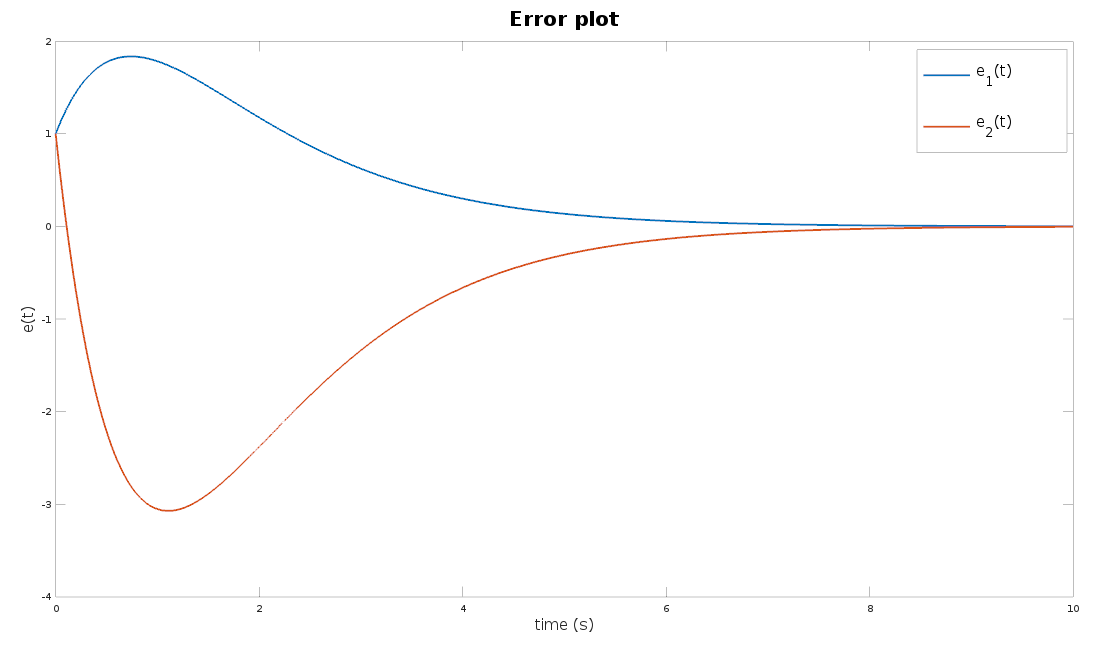
\includegraphics[scale=0.4]{q5_error_plot}
\par\end{centering}
\caption{Error plot}
\end{figure}

The code for the plot is located in the Appendix.\newpage{}

\section*{Question 6}

A system is described by the equations 

\[
\begin{aligned}\dot{X}\left(t\right)=\, & \left[\begin{array}{cc}
1 & 0\\
-5 & -20
\end{array}\right]X\left(t\right)+\left[\begin{array}{c}
100\\
0
\end{array}\right]U\left(t\right)\\
Y\left(t\right)=\, & \left[\begin{array}{cc}
1 & 0\end{array}\right]X\left(t\right)
\end{aligned}
\]
Determine observer gains to place the observer poles at $s_{1,2}=-5$.

\subsection*{Solution}

Before constructing an observer, we need to make sure that our system
is fully observable. 
\[
\begin{aligned}\left|P_{o}\right|= & \left|\begin{array}{cc}
100 & 100\\
0 & -500
\end{array}\right|\\
= & -50000\\
\neq & \,0\;\therefore\text{ fully observable}
\end{aligned}
\]

Now that we know that our system is observable, we can construct our
observer using Ackermann's formula for observability for a two-state
system, Equation \ref{eq:ackermann-eq-obs}.

\[
\begin{aligned}P_{o}^{-1}= & \,\frac{1}{\text{det}\left(P_{o}\right)}\text{adj}\left(P_{o}\right)\\
= & \,\frac{1}{-50000}\left[\begin{array}{cc}
-500 & -100\\
0 & 100
\end{array}\right]\\
= & \,\left[\begin{array}{cc}
0.01 & 0.02\\
0 & -0.2
\end{array}\right]
\end{aligned}
\]

Let's find $q\left(\lambda\right)$, which will be used to construct
$q\left(A\right)$

\[
\begin{aligned}\left(\lambda+5\right)^{2}= & \lambda^{2}+10\lambda+25=q\left(\lambda\right)\end{aligned}
\]

Therefore, 
\begin{align*}
q\left(A\right)= & A^{2}+10A+25\mathbb{I}\\
= & \left[\begin{array}{cc}
1 & 0\\
95 & 400
\end{array}\right]+10\left[\begin{array}{cc}
1 & 0\\
-5 & -20
\end{array}\right]+25\left[\begin{array}{cc}
1 & 0\\
0 & 1
\end{array}\right]\\
= & \left[\begin{array}{cc}
36 & 0\\
45 & 225
\end{array}\right]
\end{align*}

And finally
\begin{align*}
L= & q\left(A\right)P_{o}^{-1}\left[\begin{array}{cc}
0 & 1\end{array}\right]^{T}\\
= & \left[\begin{array}{cc}
36 & 0\\
45 & 225
\end{array}\right]\left[\begin{array}{cc}
0.01 & 0.02\\
0 & -0.2
\end{array}\right]\left[\begin{array}{c}
0\\
1
\end{array}\right]\\
= & \left[\begin{array}{c}
0.072\\
-0.36
\end{array}\right]
\end{align*}

Therefore, the observer gains are 
\[
\boxed{L=\left[\begin{array}{c}
0.072\\
-0.36
\end{array}\right]}
\]


\part*{Appendix}

\begin{lstlisting}
% Standard state-space matrices
A = [
 1,  4; 
-5, -10];
B = [0; 1];
C = [1, -4];
D = [0];

poles = [-1, -1];

% Need to use acker() because the poles are at the same location
% We'll use the fact that the controllability of the dual of the system
% is the same as the observability of the original system
L = acker(A' ,C',poles)';

dt = 0.001;
total_time = 10;
t = 0:dt:total_time;
num_its = length(t);

U = 1e-3; % input as a step function

X = [1; 1];       % initial states
X_hat = [0; 0];   % initial estimate of states
e0 = X - X_hat;   % initial error

% Setup vectors
X_vec = X;
X_hat_vec = X_hat;
e_vec = e0;

for i = 1:num_its-1;
  Y = C*X + D*U;
  Y_hat = C*X_hat + D*U;
  
  dX = A*X + B*U;
  X = X + dX*dt;
  
  dX_hat = A*X_hat + B*U + L*(Y - Y_hat);
  X_hat = X_hat + dX_hat*dt;
  
  e = X - X_hat;
  
  X_vec = [X_vec, X];
  X_hat_vec = [X_hat_vec, X_hat];
  e_vec = [e_vec, e];  
end

figure;

plot(t, e_vec(1,:), 'LineWidth', 2);
hold on;
plot(t, e_vec(2,:), 'LineWidth', 2);
title('Error plot', 'fontsize', 20)
xlabel('time (s)', 'fontsize', 16)
ylabel('e(t)', 'fontsize', 16)
leg = legend('e_{1}(t)', 'e_{2}(t)')
set (leg, "fontsize", 16);

% References:
% [1]: http://www.eecs.tufts.edu/~khan/Courses/Spring2013/EE194/Lecs/Lec6and7.pdf
% [2]: http://ctms.engin.umich.edu/CTMS/index.php?example=Introduction&section=ControlStateSpace#23
% [3]: http://cse.lab.imtlucca.it/~bemporad/teaching/ac/pdf/06b-estimator.pdf
\end{lstlisting}

\end{document}
